% answers.tex —— 2006 年·普通高等学校招生考试·江西卷理科 · 参考答案与详细解析片段
% 由 tools/generate_projects.py 依来源总账自 2006/2006_数学真题_江西理_试题.md + 2006/2006_数学真题_江西理_解析正文.md + 2006/2006_数学真题_江西理_答案要点.md 生成，勿手改（改源 MD 后重跑）


\begin{gktip}
以下为依据固定候选题面独立求解的草稿，不是官方答案或解析。未使用未核验的答案材料。来源身份未核；Q12 选项判断依据固定源页图象，图仍须重绘核验。
\end{gktip}

\begin{answer}
\gksolhead{1}{}

\textbf{题目}：

已知集合 $M=\left\{x\mid\dfrac{x}{(x-1)^3}\geqslant0\right\}$，$N=\{y\mid y=3x^2+1,\ x\in\mathbb R\}$，则 $M\cap N$ 等于\mbox{（　　）}

\begin{gkopts}(2)
\task （A）$\varnothing$
\task （B）$\{x\mid x\geqslant1\}$
\task （C）$\{x\mid x>1\}$
\task （D）$\{x\mid x\geqslant1\text{ \text{或} }x<0\}$
\end{gkopts}

\Needspace{4\baselineskip}
\textbf{解析}

不等式给 $M=(-\infty,0]\cup(1,+\infty)$；而 $N=[1,+\infty)$。故 $M\cap N=(1,+\infty)$，选 C。

\gkanswer{答案：C。}

\end{answer}
\begin{answer}
\gksolhead{2}{}

\textbf{题目}：

已知复数 $z$ 满足 $(\sqrt3+3i)z=3i$，则 $z$ 等于\mbox{（　　）}

\begin{gkopts}(2)
\task （A）$\dfrac32-\dfrac{\sqrt3}{2}i$
\task （B）$\dfrac34-\dfrac{\sqrt3}{4}i$
\task （C）$\dfrac32+\dfrac{\sqrt3}{2}i$
\task （D）$\dfrac34+\dfrac{\sqrt3}{4}i$
\end{gkopts}

\Needspace{4\baselineskip}
\textbf{解析}

\nopagebreak[4]
\[
z=\frac{3i}{\sqrt3+3i}=\frac{3i(\sqrt3-3i)}{12}=\frac34+\frac{\sqrt3}{4}i,
\]

选 D。

\gkanswer{答案：D。}

\end{answer}
\begin{answer}
\gksolhead{3}{}

\textbf{题目}：

若 $a>0\text{，}b>0$，则不等式 $-b<\dfrac1x<a$ 等价于\mbox{（　　）}

（A）$-\dfrac1b<x<0$ 或 $0<x<\dfrac1a$　（B）$-\dfrac1a<x<\dfrac1b$

（C）$x<-\dfrac1a$ 或 $x>\dfrac1b$　（D）$x<-\dfrac1b$ 或 $x>\dfrac1a$

\Needspace{4\baselineskip}
\textbf{解析}

若 $x>0$，则 $1/x<a$ 给 $x>1/a$，而 $-b<1/x$ 自动成立；若 $x<0$，则 $-b<1/x$ 给 $x<-1/b$，另一不等式自动成立。$x=0$ 不在定义域，故选 D。

\gkanswer{答案：D。}

\end{answer}
\begin{answer}
\gksolhead{4}{}

\textbf{题目}：

设 $O$ 为坐标原点，$F$ 为抛物线 $y^2=4x$ 的焦点，$A$ 为抛物线上的一点，若 $\overrightarrow{OA}\cdot\overrightarrow{AF}=-4$，则点 $A$ 的坐标为\mbox{（　　）}

\begin{gkopts}(2)
\task （A）$(2,\pm2\sqrt2)$
\task （B）$(1,\pm2)$
\task （C）$(1,2)$
\task （D）$(2,2\sqrt2)$
\end{gkopts}

\Needspace{4\baselineskip}
\textbf{解析}

抛物线焦点为 $F=(1,0)$。设 $A=(x,y)$ 且 $y^2=4x$，则 $\overrightarrow{OA}\cdot\overrightarrow{AF}=x(1-x)-y^2=-4$，化为 $x^2+3x-4=0$。结合 $x\ge0$ 得 $x=1$、$y=\pm2$，选 B。

\gkanswer{答案：B。}

\end{answer}
\begin{answer}
\gksolhead{5}{}

\textbf{题目}：

对于 $\mathbb R$ 上可导的任意函数 $f(x)$，若满足 $(x-1)f'(x)\geqslant0$，则必有\mbox{（　　）}

\begin{gkopts}(2)
\task （A）$f(0)+f(2)<2f(1)$
\task （B）$f(0)+f(2)\leqslant2f(1)$
\task （C）$f(0)+f(2)\geqslant2f(1)$
\task （D）$f(0)+f(2)>2f(1)$
\end{gkopts}

\Needspace{4\baselineskip}
\textbf{解析}

在 $x<1$ 上 $f'(x)\le0$，故 $f(0)\ge f(1)$；在 $x>1$ 上 $f'(x)\ge0$，故 $f(2)\ge f(1)$。相加得 $f(0)+f(2)\ge2f(1)$，选 C。

\gkanswer{答案：C（5 项）。}

\end{answer}
\begin{answer}
\gksolhead{6}{}

\textbf{题目}：

若不等式 $x^2+ax+1\geqslant0$ 对一切 $x\in\left(0,\dfrac12\right]$ 成立，则 $a$ 的最小值为\mbox{（　　）}

\begin{gkopts}(4)
\task （A）$0$
\task （B）$-2$
\task （C）$-\dfrac52$
\task （D）$-3$
\end{gkopts}

\Needspace{4\baselineskip}
\textbf{解析}

对 $x>0$，条件等价于 $a\ge-x-1/x$。在 $(0,1/2]$ 上，$-x-1/x$ 的最大值为其端点值 $-5/2$，故 $a$ 的最小值是 $-5/2$，选 C。

\gkanswer{答案：C（$-5/2$）。}

\end{answer}
\begin{answer}
\gksolhead{7}{}

\textbf{题目}：

已知等差数列 $\{a_n\}$ 的前 $n$ 项和为 $S_n$，若 $\overrightarrow{OB}=a_1\overrightarrow{OA}+a_{200}\overrightarrow{OC}$，且 $A\text{、}B\text{、}C$ 三点共线（该直线不过点 $O$），则 $S_{200}$ 等于\mbox{（　　）}

\begin{gkopts}(4)
\task （A）$100$
\task （B）$101$
\task （C）$200$
\task （D）$201$
\end{gkopts}

\Needspace{4\baselineskip}
\textbf{解析}

设 $A=(u,0),B=(0,v),P=(x,y)$。由 $\overrightarrow{BP}=2\overrightarrow{PA}$ 得 $3P=2A+B$，所以 $u=3x/2,v=3y$。又 $Q=(-x,y)$，从 $\overrightarrow{OQ}\cdot\overrightarrow{AB}=1$ 得 $xu+yv=1$。代入即 $3x^2/2+3y^2=1$，选 D。

\gkanswer{答案：D。}

\end{answer}
\begin{answer}
\gksolhead{8}{}

\textbf{题目}：

在 $(x-\sqrt2)^{2006}$ 的二项展开式中，含 $x$ 的奇次幂的项之和为 $S$，当 $x=\sqrt2$ 时，$S$ 等于\mbox{（　　）}

\begin{gkopts}(4)
\task （A）$2^{3008}$
\task （B）$-2^{3008}$
\task （C）$2^{3009}$
\task （D）$-2^{3009}$
\end{gkopts}

\Needspace{4\baselineskip}
\textbf{解析}

①由 $|A\cup B|=|A|+|B|-|A\cap B|$ 成立；②是包含关系的必要条件；③可取 $A=B$ 且基数相等反例；④同基数集合不必相等。真命题为①②，选 B。

\gkanswer{答案：B。}

\end{answer}
\begin{answer}
\gksolhead{9}{}

\textbf{题目}：

$P$ 为双曲线 $\dfrac{x^2}{9}-\dfrac{y^2}{16}=1$ 的右支上一点，$M\text{、}N$ 分别是圆 $(x+5)^2+y^2=4$ 和 $(x-5)^2+y^2=1$ 上的点，则 $|PM|-|PN|$ 的最大值为\mbox{（　　）}

\begin{gkopts}(4)
\task （A）$6$
\task （B）$7$
\task （C）$8$
\task （D）$9$
\end{gkopts}

\Needspace{4\baselineskip}
\textbf{解析}

双曲线焦点为 $(-5,0),(5,0)$，离焦点的距离差在右支恒为 $6$。取 $M,N$ 分别为两圆上使 $PM$ 最大、$PN$ 最小的点，距离差在双曲线差值上再增加两半径 $2+1$，最大为 $6+2+1=9$，选 D。

\gkanswer{答案：D（9）。}

\end{answer}
\begin{answer}
\gksolhead{10}{}

\textbf{题目}：

将 7 个人（含甲、乙）分成三组，一组 3 人，另两组各 2 人，不同的分组数为 $a$，甲、乙分在同一组的概率为 $p$，则 $a\text{、}p$ 的值分别为\mbox{（　　）}

（A）$a=105\text{，}p=\dfrac5{21}$　（B）$a=105\text{，}p=\dfrac4{21}$

（C）$a=210\text{，}p=\dfrac5{21}$　（D）$a=210\text{，}p=\dfrac4{21}$

\Needspace{4\baselineskip}
\textbf{解析}

总分组数为 $\binom73\cdot3=105$。甲乙同在三人组时有 $5\cdot3=15$ 种；同在二人组时有 $\binom52=10$ 种，共 $25$ 种。因此 $p=25/105=5/21$，选 A。

\gkanswer{答案：A（$a=105,\ p=5/21$）。}

\end{answer}
\begin{answer}
\gksolhead{11}{}

\textbf{题目}：

如图，在四面体 $ABCD$ 中，截面 $AEF$ 经过四面体的内切球（与四个面都相切的球）球心 $O$，且与 $BC\text{、}DC$ 分别截于 $E\text{、}F$。如果截面将四面体分为体积相等的两部分，设四棱锥 $A-BEFD$ 与三棱锥 $A-EFC$ 的表面积分别为 $S_1\text{、}S_2$，则必有\mbox{（　　）}

\begin{gkopts}(2)
\task （A）$S_1<S_2$
\task （B）$S_1>S_2$
\task （C）$S_1=S_2$
\task （D）$S_1\text{、}S_2$ 的大小不能确定
\end{gkopts}
\nopagebreak[4]
\begin{center}% Q11：按固定候选 PDF 第 1 页可见关系重绘。空间位置为示意，不表示比例。
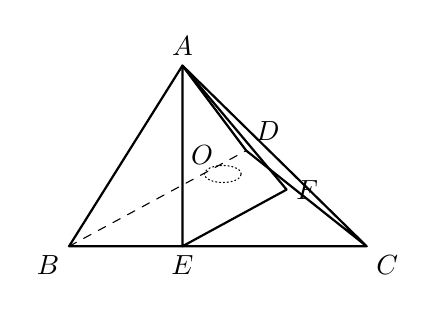
\begin{tikzpicture}[line cap=round,line join=round,scale=0.9]
  \coordinate (A) at (-0.55,2.55);
  \coordinate (B) at (-2.15,0);
  \coordinate (C) at (2.05,0);
  \coordinate (D) at (0.35,1.35);
  \coordinate (E) at (-0.55,0);
  \coordinate (F) at (0.92,0.80);
  \coordinate (O) at (0.02,1.02);

  % 四面体棱与截面；隐藏的棱以虚线表示。
  \draw[thick] (A)--(B) (B)--(C) (C)--(A) (A)--(D) (D)--(C);
  \draw[dashed] (B)--(D);
  \draw[thick] (A)--(E) (E)--(F) (F)--(A);
  % 截面内切球的圆截面，仅表示球心与相切关系，不表示比例。
  \draw[densely dotted] (O) ellipse (0.26 and 0.12);

  \node[above] at (A) {$A$};
  \node[below left] at (B) {$B$};
  \node[below right] at (C) {$C$};
  \node[above right] at (D) {$D$};
  \node[below] at (E) {$E$};
  \node[right] at (F) {$F$};
  \node[above left] at (O) {$O$};
\end{tikzpicture}
\end{center}
\nopagebreak[4]
\Needspace{4\baselineskip}
\textbf{解析}

令截平面为仿射函数零面，并设 $\ell(A)=0,\ell(B)=p,\ell(C)=-c,\ell(D)=q$，其中 $p,c,q>0$。记 $u=CE/CB=c/(p+c)$、$v=CF/CD=c/(q+c)$。截面切出的底面三角形 $EFC$ 面积占 $BCD$ 的比例为 $uv$；两部分等体积给 $uv=1/2$。

\Needspace{5\baselineskip}
记 $T_A,T_B,T_C,T_D$ 为原四面体各顶点对面面积。内心的重心坐标与对面面积成正比，且 $\ell(O)=0$，所以 $pT_B-cT_C+qT_D=0$，即
\nopagebreak[4]
\[
T_C=T_B\frac{1-u}{u}+T_D\frac{1-v}{v}.
\]

\Needspace{5\baselineskip}
两块立体的共同截面 $AEF$ 在表面积差中抵消。底面差为 $[BEFD]-[EFC]=(1-2uv)T_A=0$；侧面分割给 $[ABE]-[AEC]=(1-2u)T_D$、$[AFD]-[ACF]=(1-2v)T_B$。故
\nopagebreak[4]
\[
S_1-S_2=T_B(1/u-2v)+T_D(1/v-2u)=0,
\]

其中用到了 $uv=1/2$。所以 $S_1=S_2$，选 C。

\gkanswer{答案：C（$S_1=S_2$）。}

\end{answer}
\begin{answer}
\gksolhead{12}{}

\textbf{题目}：

某地一年内的气温 $Q(t)$（单位：$^\circ\mathrm C$）与时间 $t$（月份）之间的关系如图所示，已知该年的平均气温为 $10\ ^\circ\mathrm C$。令 $C(t)$ 表示时间段 $[0,t]$ 的平均气温，$C(t)$ 与 $t$ 之间的函数关系用下列图象表示，则正确的是\mbox{（　　）}
\nopagebreak[4]
\begin{center}% Q12：依固定候选 PDF 第 1 页重绘温度曲线与四个选项；曲线为定性示意。
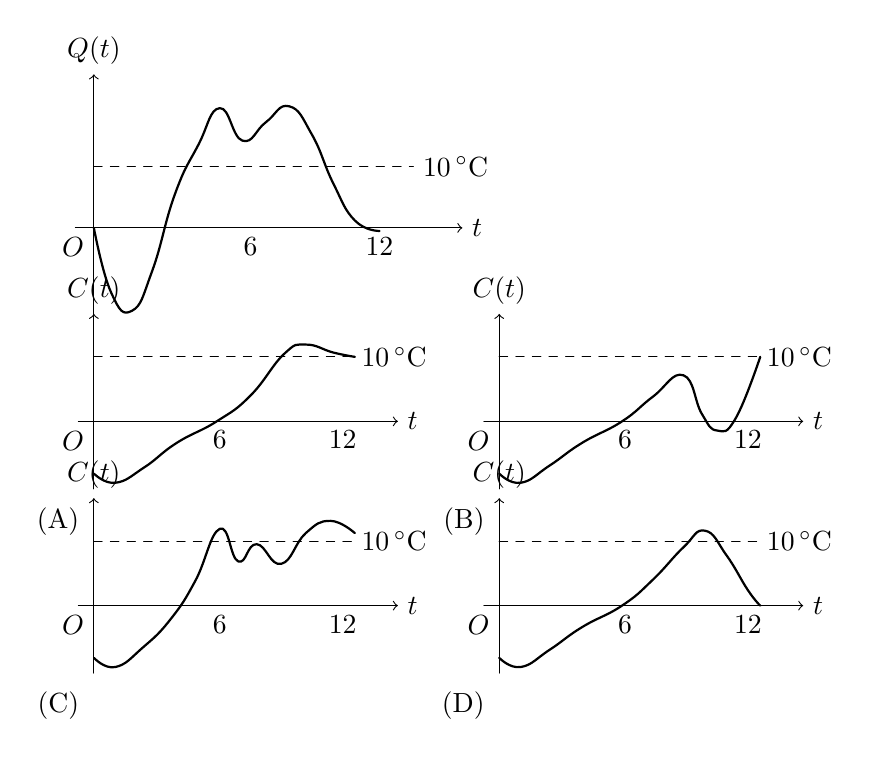
\begin{tikzpicture}[line cap=round,line join=round,scale=0.78]
  % 顶部：气温 Q(t)
  \begin{scope}[shift={(0,5.7)}]
    \draw[->] (-0.3,0)--(6.0,0) node[right] {$t$};
    \draw[->] (0,-1.55)--(0,2.5) node[above] {$Q(t)$};
    \draw[dashed] (0,1.0)--(5.2,1.0) node[right] {$10\,{}^\circ\mathrm C$};
    \draw[thick] plot[smooth,tension=0.82] coordinates
      {(0,0) (0.28,-1.05) (0.62,-1.35) (0.95,-0.7) (1.32,0.55)
       (1.7,1.35) (2.05,1.95) (2.42,1.42) (2.8,1.72) (3.18,1.98)
       (3.55,1.52) (3.9,0.72) (4.25,0.12) (4.65,-0.05)};
    \node[below left] at (0,0) {$O$};
    \node[below] at (2.55,0) {$6$};
    \node[below] at (4.65,0) {$12$};
  \end{scope}

  % 四个选项共用坐标尺度；各曲线只表达原图趋势。
  \foreach \x/\y/\letter in {0/2.55/A,6.6/2.55/B,0/-0.45/C,6.6/-0.45/D}{
    \begin{scope}[shift={(\x,\y)}]
      \draw[->] (-0.25,0)--(4.95,0) node[right] {$t$};
      \draw[->] (0,-1.1)--(0,1.75) node[above] {$C(t)$};
      \draw[dashed] (0,1.05)--(4.2,1.05) node[right] {$10\,{}^\circ\mathrm C$};
      \node[below left] at (0,0) {$O$};
      \node[below] at (2.05,0) {$6$};
      \node[below] at (4.05,0) {$12$};
      \node[below left] at (-0.08,-1.25) {(\letter)};
    \end{scope}
  }
  % (A) 先下降，约在 6 月穿过 0，之后高于 10，最后回到 10。
  \begin{scope}[shift={(0,2.55)}]
    \draw[thick] plot[smooth,tension=0.8] coordinates
      {(0,-0.85) (0.35,-1.0) (0.82,-0.75) (1.35,-0.35)
       (2.0,0) (2.55,0.42) (3.1,1.1) (3.45,1.25)
       (3.9,1.12) (4.25,1.05)};
  \end{scope}
  % (B) 先下降，约在 6 月穿过 0，之后略降至 0 以下再升到 10。
  \begin{scope}[shift={(6.6,2.55)}]
    \draw[thick] plot[smooth,tension=0.8] coordinates
      {(0,-0.85) (0.35,-1.0) (0.82,-0.72) (1.35,-0.35)
       (2.0,0) (2.5,0.4) (3.0,0.75) (3.3,0.12)
       (3.55,-0.15) (3.85,0.05) (4.25,1.05)};
  \end{scope}
  % (C) 先上升越过 10，随后起伏，末端仍在 10 上方。
  \begin{scope}[shift={(0,-0.45)}]
    \draw[thick] plot[smooth,tension=0.8] coordinates
      {(0,-0.85) (0.35,-1.0) (0.8,-0.68) (1.25,-0.22)
       (1.65,0.4) (2.05,1.25) (2.35,0.72) (2.65,1.0)
       (3.05,0.68) (3.45,1.18) (3.85,1.38) (4.25,1.18)};
  \end{scope}
  % (D) 先下降，约在 6 月穿过 0，形成高于 10 的峰后于 12 月回到 0。
  \begin{scope}[shift={(6.6,-0.45)}]
    \draw[thick] plot[smooth,tension=0.8] coordinates
      {(0,-0.85) (0.35,-1.0) (0.82,-0.72) (1.35,-0.35)
       (2.0,0) (2.5,0.42) (3.0,0.95) (3.35,1.22)
       (3.7,0.82) (4.05,0.25) (4.25,0)};
  \end{scope}
\end{tikzpicture}
\end{center}
\nopagebreak[4]
\Needspace{4\baselineskip}
\textbf{解析}

$C(t)=t^{-1}\int_0^tQ(s)\,ds$，故 $C(12)=10$，排除末值不为 $10$ 的图 C、D。源图中在 $t$ 从 $6$ 到约 $10$ 的阶段，$Q(t)$ 高于当时的平均值 $C(t)$，于是 $C'(t)=(Q(t)-C(t))/t>0$，排除在该段出现先升后降小波谷的图 B。符合起始下降、之后上升并在 $t=12$ 回到 $10$ 的是 A。

\gkanswer{答案：A。}

\end{answer}
\begin{answer}
\gksolhead{13}{}

\textbf{题目}：

数列 $\left\{\dfrac1{4n^2-1}\right\}$ 的前 $n$ 项和为 $S_n$，则 $\lim_{n\to\infty}S_n=$ \gkblank{}。

\Needspace{4\baselineskip}
\textbf{解析}

\nopagebreak[4]
\[
\frac1{4n^2-1}=\frac12\left(\frac1{2n-1}-\frac1{2n+1}\right).
\]

故 $S_n=\frac12(1-1/(2n+1))$，极限为 $1/2$。

\gkanswer{答案：$1/2$。}

\end{answer}
\begin{answer}
\gksolhead{14}{}

\textbf{题目}：

设 $f(x)=\log_3(x+6)$ 的反函数为 $f^{-1}(x)$，若 $[f^{-1}(m)+6]\cdot[f^{-1}(n)+6]=27$，则 $f(m+n)=$ \gkblank{}。

\Needspace{4\baselineskip}
\textbf{解析}

$f^{-1}(x)=3^x-6$，因此 $f^{-1}(m)+6=3^m$、$f^{-1}(n)+6=3^n$。题设给 $3^{m+n}=27$，所以 $m+n=3$，$f(m+n)=\log_3 9=2$。

\gkanswer{答案：$2$。}

\end{answer}
\begin{answer}
\gksolhead{15}{}

\textbf{题目}：

如图，在直三棱柱 $ABC-A_1B_1C_1$ 中，底面为直角三角形，$\angle ACB=90^\circ$，$AC=6\text{，}BC=CC_1=\sqrt2$，$P$ 是 $BC_1$ 上一动点，则 $CP+PA_1$ 的最小值为 \gkblank{}。
\nopagebreak[4]
\begin{center}% Q15：按固定候选 PDF 第 1 页重绘直三棱柱及 P 的位置；透视比例为示意。
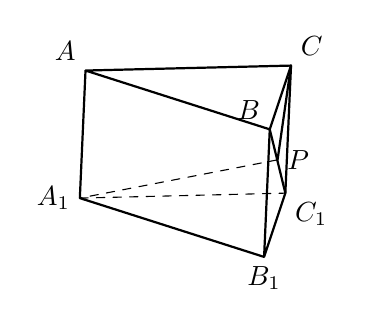
\begin{tikzpicture}[line cap=round,line join=round,scale=0.9]
  \coordinate (A) at (-1.75,1.55);
  \coordinate (B) at (0.85,0.72);
  \coordinate (C) at (1.15,1.62);
  \coordinate (A1) at (-1.83,-0.25);
  \coordinate (B1) at (0.77,-1.08);
  \coordinate (C1) at (1.07,-0.18);
  \coordinate (P) at (0.96,0.29);

  % 棱线；底部后侧棱 A1C1 按原图用虚线。
  \draw[thick] (A)--(B)--(C)--(A) (A)--(A1) (B)--(B1) (C)--(C1)
    (A1)--(B1)--(C1);
  \draw[dashed] (A1)--(C1);
  % BC1 上的动点 P，以及题目中的线段。
  \draw[thick] (B)--(C1) (C)--(P);
  \draw[dashed] (P)--(A1);

  \node[above left] at (A) {$A$};
  \node[above left] at (B) {$B$};
  \node[above right] at (C) {$C$};
  \node[left] at (A1) {$A_1$};
  \node[below] at (B1) {$B_1$};
  \node[below right] at (C1) {$C_1$};
  \node[right] at (P) {$P$};
\end{tikzpicture}
\end{center}
\nopagebreak[4]
\Needspace{4\baselineskip}
\textbf{解析}

\Needspace{5\baselineskip}
取 $C=(0,0,0),B=(\sqrt2,0,0),A=(0,6,0),A_1=(0,6,\sqrt2)$，令 $P=(\sqrt2u,0,\sqrt2(1-u))$，$0\le u\le1$。则
\nopagebreak[4]
\[
CP=\sqrt{4u^2-4u+2},\qquad PA_1=\sqrt{36+4u^2}.
\]

对两者之和求导，驻点为 $u=3/7$，且为区间内唯一极小点。两段长度分别为 $5\sqrt2/7$ 与 $30\sqrt2/7$，最小和为 $5\sqrt2$。

\gkanswer{答案：$5\sqrt2$。}

\end{answer}
\begin{answer}
\gksolhead{16}{}

\textbf{题目}：

已知圆 $M:(x+\cos\theta)^2+(y-\sin\theta)^2=1$，直线 $l:y=kx$，下面四个命题：

① 对任意实数 $k$ 和 $\theta$，直线 $l$ 和圆 $M$ 相切；

② 对任意实数 $k$ 和 $\theta$，直线 $l$ 和圆 $M$ 有公共点；

③ 对任意实数 $\theta$，必存在实数 $k$，使得直线 $l$ 和圆 $M$ 相切；

④ 对任意实数 $k$，必存在实数 $\theta$，使得直线 $l$ 和圆 $M$ 相切。

其中真命题的代号是 \gkblank{}。（写出所有真命题的代号）

\Needspace{4\baselineskip}
\textbf{解析}

\Needspace{5\baselineskip}
圆心为 $(-\cos\theta,\sin\theta)$，半径为 $1$。任意过原点直线到该圆心距离不超过 $1$，故直线与圆必有公共点，②真。相切等价于
\nopagebreak[4]
\[
(k\sin\theta-\cos\theta)^2=0.
\]

对某些 $\theta$（如 $\theta=0$）不存在有限 $k$，所以③假；对任意 $k$ 可选 $\theta$ 使 $k\sin\theta=\cos\theta$，故④真。①显然不对所有 $k,\theta$ 成立。答案为②④。

\gkanswer{答案：②④。}

\end{answer}
\begin{answer}
\gksolhead{17}{}

\textbf{题目}：

已知函数 $f(x)=x^3+ax^2+bx+c$ 在 $x=-\dfrac23$ 与 $x=1$ 时都取得极值。

(1) 求 $a\text{、}b$ 的值与函数 $f(x)$ 的单调区间；

(2) 若对 $x\in[-1,2]$，不等式 $f(x)<c^2$ 恒成立，求 $c$ 的取值范围。

\Needspace{4\baselineskip}
\textbf{解析}

\gksubpart{(1)}

$f'(x)=3x^2+2ax+b$ 的两根为 $-2/3,1$，比较系数得 $a=-1/2,b=-2$。因此 $f'(x)=3(x+2/3)(x-1)$，得到所列单调区间。

\gksubpart{(2)}

写 $f(x)=x^3-x^2/2-2x+c$。在 $[-1,2]$ 上，不含 $c$ 的部分最大值为 $2$（在 $x=2$ 取得）。恒成立条件化为 $2+c<c^2$，故 $c<-1$ 或 $c>2$。

\gkanswer{答案（1）：$a=-1/2,\ b=-2$；递增区间 $(-\infty,-2/3)$、$(1,+\infty)$，递减区间 $(-2/3,1)$。}

\gkanswer{答案（2）：$c<-1$ 或 $c>2$。}

\end{answer}
\begin{answer}
\gksolhead{18}{}

\textbf{题目}：

某商场举行抽奖促销互动，抽奖规则是：从装有 9 个白球、1 个红球的箱子中每次随机地摸出一个球，记下颜色后放回，摸出一个红球可获得奖金 10 元；摸出两个红球可获得奖金 50 元。现有甲、乙两位顾客，规定：甲摸一次，乙摸两次。令 $\xi$ 表示甲、乙两人摸球后获得的奖金总额。求：

(1) $\xi$ 的分布列；

(2) $\xi$ 的数学期望。

\Needspace{4\baselineskip}
\textbf{解析}

\gksubpart{(1)}

甲所得奖金为 $0,10$，概率为 $0.9,0.1$；乙所得奖金为 $0,10,50$，概率为 $0.81,0.18,0.01$。独立卷积得总奖金 $0,10,20,50,60$ 的概率依次为 $729,243,18,9,1$ 除以 $1000$。

\gksubpart{(2)}

$E(\xi)=10(0.1)+10(0.18)+50(0.01)=3.3$ 元。

\gkanswer{答案（1）：$\xi$ 取 $0,10,20,50,60$ 的概率依次为 $729/1000,243/1000,18/1000,9/1000,1/1000$。}

\gkanswer{答案（2）：$E(\xi)=33/10$ 元。}

\end{answer}
\begin{answer}
\gksolhead{19}{}

\textbf{题目}：

如图，已知 $\triangle ABC$ 是边长为 1 的正三角形，$M\text{、}N$ 分别是边 $AB\text{、}AC$ 上的点，线段 $MN$ 经过 $\triangle ABC$ 的中心 $G$。设 $\angle MGA=\alpha\ \left(\dfrac\pi3\leqslant\alpha\leqslant\dfrac{2\pi}3\right)$。

(1) 试将 $\triangle AGM\text{、}\triangle AGN$ 的面积（分别记为 $S_1$ 与 $S_2$）表示为 $\alpha$ 的函数；

(2) 求 $y=\dfrac1{S_1^2}+\dfrac1{S_2^2}$ 的最大值与最小值。
\nopagebreak[4]
\begin{center}% Q19：按固定候选 PDF 第 2 页重绘正三角形、中心、MN 与角 alpha；不表示精确比例。
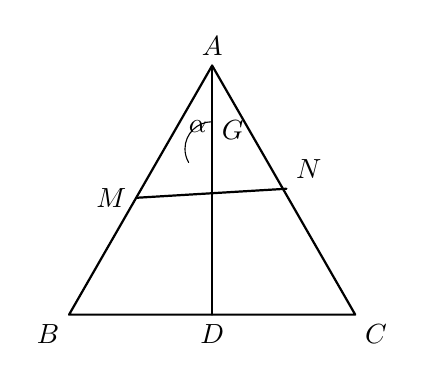
\begin{tikzpicture}[line cap=round,line join=round,scale=1.15]
  \coordinate (A) at (0,2.75);
  \coordinate (B) at (-1.58,0);
  \coordinate (C) at (1.58,0);
  \coordinate (D) at (0,0);
  \coordinate (G) at (0,1.83);
  \coordinate (M) at (-0.84,1.29);
  \coordinate (N) at (0.82,1.39);

  \draw[thick] (A)--(B)--(C)--cycle;
  \draw[thick] (A)--(D);
  \draw[thick] (M)--(N);
  \draw (G) ++(90:0.30) arc[start angle=90,end angle=210,radius=0.30];

  \node[above] at (A) {$A$};
  \node[below left] at (B) {$B$};
  \node[below right] at (C) {$C$};
  \node[below] at (D) {$D$};
  \node[above right] at (G) {$G$};
  \node[left] at (M) {$M$};
  \node[above right] at (N) {$N$};
  \node at (-0.16,2.08) {$\alpha$};
\end{tikzpicture}
\end{center}
\nopagebreak[4]
\Needspace{4\baselineskip}
\textbf{解析}

\gksubpart{(1)}

\Needspace{5\baselineskip}
正三角形中心 $G$ 到顶点的距离为 $AG=\sqrt3/3$。由图中角关系及正弦定理，
\nopagebreak[4]
\[
S_1=\frac{\sin\alpha}{12\sin(150^\circ-\alpha)},\qquad
S_2=\frac{\sin\alpha}{12\sin(\alpha-30^\circ)}.
\]

\gksubpart{(2)}

化简得 $y=144(1+1/(1-\cos2\alpha))$。区间 $\alpha\in[60^\circ,120^\circ]$ 上 $\cos2\alpha\in[-1,-1/2]$，故最小值 $216$（$\alpha=90^\circ$），最大值 $240$（区间端点）。

\gkanswer{答案（1）：$S_1=\frac{\sin\alpha}{12\sin(150^\circ-\alpha)}$，$S_2=\frac{\sin\alpha}{12\sin(\alpha-30^\circ)}$。}

\gkanswer{答案（2）：最大值 $240$，最小值 $216$。}

\end{answer}
\begin{answer}
\gksolhead{20}{}

\textbf{题目}：

如图，在三棱锥 $A-BCD$ 中，侧面 $ABD\text{、}ACD$ 是全等的直角三角形，$AD$ 是公共的斜边，且 $AD=\sqrt3\text{，}BD=CD=1$，另一个侧面 $ABC$ 是正三角形。

(1) 求证：$AD\perp BC$；

(2) 求二面角 $B-AC-D$ 的大小；

(3) 在直线 $AC$ 上是否存在一点 $E$，使 $ED$ 与面 $BCD$ 成 $30^\circ$ 角？若存在，确定 $E$ 的位置；若不存在，说明理由。
\nopagebreak[4]
\begin{center}% Q20：按固定候选 PDF 第 2 页重绘三棱锥；空间位置为示意，不补入长度或角度标记。
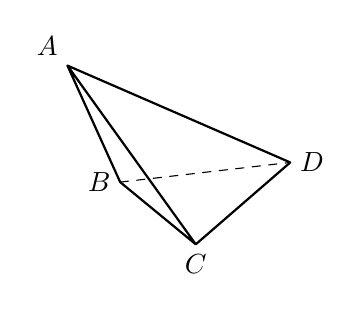
\begin{tikzpicture}[line cap=round,line join=round,scale=1.0]
  \coordinate (A) at (-1.45,1.95);
  \coordinate (B) at (-0.78,0.47);
  \coordinate (C) at (0.18,-0.32);
  \coordinate (D) at (1.38,0.72);

  % 原图中 BD 为隐藏棱，其余外轮廓与侧棱为实线。
  \draw[thick] (A)--(B) (A)--(C) (A)--(D) (B)--(C) (C)--(D);
  \draw[dashed] (B)--(D);

  \node[above left] at (A) {$A$};
  \node[left] at (B) {$B$};
  \node[below] at (C) {$C$};
  \node[right] at (D) {$D$};
\end{tikzpicture}
\end{center}
\nopagebreak[4]
\Needspace{4\baselineskip}
\textbf{解析}

\gksubpart{(1)}

$AB=AC=BC=\sqrt2$ 且 $DB=DC=1$，所以 $A,D$ 都在 $BC$ 的垂直平分面上，得到 $AD\perp BC$。

\gksubpart{(2)}

\Needspace{5\baselineskip}
以 $BC$ 中点为原点建立坐标系，可取
\nopagebreak[4]
\[
B=(-1/\sqrt2,0,0),\ C=(1/\sqrt2,0,0),\ A=(0,\sqrt6/2,0),\ D=(0,-1/\sqrt6,1/\sqrt3).
\]

用 $AC,AB$ 所在平面的法向量计算，二面角余弦为 $\sqrt{2/3}$。

\gksubpart{(3)}

令 $E=A+t(C-A)$。计算点 $D$ 到平面 $BCD$ 的有向垂直距离与 $ED$ 长度，线面角正弦为 $|1-t|/\sqrt{2t^2-4t+3}$。令其等于 $1/2$，得 $t=1\pm\sqrt2/2$，故直线 $AC$ 上有两点满足条件。

\gkanswer{答案（1）：$AD\perp BC$。}

\gkanswer{答案（2）：二面角 $B-AC-D$ 为 $\arccos\sqrt{2/3}$。}

\gkanswer{答案（3）：存在两点；若 $E=A+t(C-A)$，则 $t=1\pm\sqrt2/2$。}

\end{answer}
\begin{answer}
\gksolhead{21}{}

\textbf{题目}：

如图，椭圆 $Q:\dfrac{x^2}{a^2}+\dfrac{y^2}{b^2}=1\ (a>b>0)$ 的右焦点为 $F(c,0)$，过点 $F$ 的一动直线 $m$ 绕点 $F$ 转动，并且交椭圆于 $A\text{、}B$ 两点，$P$ 为线段 $AB$ 的中点。

(1) 求点 $P$ 的轨迹 $H$ 的方程；

(2) 在 $Q$ 的方程中，令 $a^2=1+\cos\theta+\sin\theta\text{，}b^2=\sin\theta\ \left(0<\theta\leqslant\dfrac\pi2\right)$，确定 $\theta$ 的值，使原点距椭圆的右准线 $l$ 最远，此时，设 $l$ 与 $x$ 轴交点为 $D$，当直线 $m$ 绕点 $F$ 转动到什么位置时，三角形 $ABD$ 的面积最大？
\nopagebreak[4]
\begin{center}% Q21：按固定候选 PDF 第 2 页重绘椭圆、弦 AB、中点 P、过 F 的直线 m 与右准线 l；比例为示意。
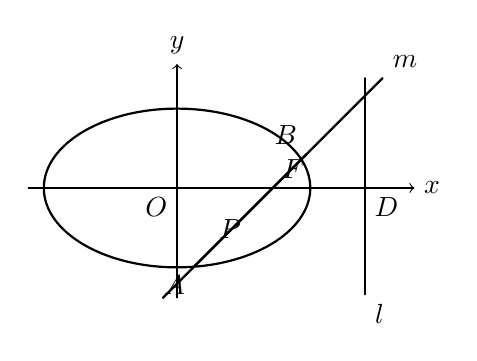
\begin{tikzpicture}[line cap=round,line join=round,scale=0.9]
  \coordinate (O) at (0,0);
  \coordinate (F) at (1.35,0);
  \coordinate (D) at (2.65,0);
  \coordinate (A) at (0.25,-1.10);
  \coordinate (B) at (1.83,0.48);
  \coordinate (P) at (1.04,-0.31);

  \draw[->] (-2.1,0)--(3.35,0) node[right] {$x$};
  \draw[->] (0,-1.55)--(0,1.75) node[above] {$y$};
  \draw[thick] (O) ellipse (1.88 and 1.12);
  \draw[thick] (-0.2,-1.55)--(2.9,1.55) node[above right] {$m$};
  \draw[thick] (A)--(B);
  \draw[thick] (2.65,-1.5)--(2.65,1.55) node[below right] at (2.65,-1.5) {$l$};

  \node[below left] at (O) {$O$};
  \node[above right] at (F) {$F$};
  \node[above left] at (B) {$B$};
  \node[below left] at (A) {$A$};
  \node[below left] at (P) {$P$};
  \node[below right] at (D) {$D$};
\end{tikzpicture}
\end{center}
\nopagebreak[4]
\Needspace{4\baselineskip}
\textbf{解析}

\gksubpart{(1)}

\Needspace{5\baselineskip}
设椭圆上弦端点为 $P\pm v$。将两端点代入椭圆方程并相减，可得弦中点 $P$ 满足 $P^{\mathsf T}\operatorname{diag}(a^{-2},b^{-2})v=0$。又弦所在直线过焦点 $F(c,0)$，故 $P,F,v$ 共线，整理得轨迹方程
\nopagebreak[4]
\[
\frac{x^2}{a^2}+\frac{y^2}{b^2}=\frac{cx}{a^2}.
\]

\gksubpart{(2)}

\Needspace{5\baselineskip}
焦距 $c=\sqrt{1+\cos\theta}$，右准线到原点的距离为 $a^2/c=\sqrt{1+\cos\theta}+\sqrt{1-\cos\theta}$，其平方为 $2+2\sin\theta$，在给定范围于 $\theta=\pi/2$ 最大。此时椭圆 $x^2/2+y^2=1$，焦点 $F=(1,0)$，右准线为 $x=2$，$D=(2,0)$。令过 $F$ 的弦斜率为 $k$，可得
\nopagebreak[4]
\[
[ABD]=\frac{\sqrt2|k|\sqrt{1+k^2}}{1+2k^2}\le\frac1{\sqrt2},
\]

等号由竖直弦 $x=1$ 取得。

\gkanswer{答案（1）：点 $P$ 的轨迹方程为 $\frac{x^2}{a^2}+\frac{y^2}{b^2}=\frac{cx}{a^2}$。}

\gkanswer{答案（2）：$\theta=\pi/2$；此时 $m$ 为 $x=1$，三角形面积最大值为 $1/\sqrt2$。}

\end{answer}
\begin{answer}
\gksolhead{22}{}

\textbf{题目}：

已知数列 $\{a_n\}$ 满足：$a_1=\dfrac32$，且 $a_n=\dfrac{3na_{n-1}}{2a_{n-1}+n-1}\ (n\geqslant2\text{，}n\in\mathbb N^*)$。

(1) 求数列 $\{a_n\}$ 的通项公式；

(2) 证明：对一切正整数 $n$，不等式 $a_1\cdot a_2\cdots a_n<2\cdot n!$ 恒成立。

\Needspace{4\baselineskip}
\textbf{解析}

\gksubpart{(1)}

令 $b_n=n/a_n$。原递推化为 $b_n=2/3+b_{n-1}/3$，且 $b_1=2/3$，故 $b_n=1-3^{-n}$，从而 $a_n=n/(1-3^{-n})$。

\gksubpart{(2)}

\Needspace{5\baselineskip}
因此
\nopagebreak[4]
\[
\frac{a_1a_2\cdots a_n}{n!}=\prod_{k=1}^n(1-3^{-k})^{-1}.
\]

有限乘积满足 $\prod_{k=1}^n(1-3^{-k})>1-\sum_{k=1}^n3^{-k}>1/2$，故所求乘积小于 $2n!$。

\gkanswer{答案（1）：$a_n=\frac{n}{1-3^{-n}}=\frac{n3^n}{3^n-1}$。}

\gkanswer{答案（2）：见解析版}

\end{answer}